\documentclass[a4paper,12pt]{article}
\usepackage{CJKutf8}
\usepackage{amsthm}
\usepackage{amsmath}
\usepackage{amssymb}
\usepackage{geometry}
\usepackage{tikz}
\usepackage{tkz-euclide}
\usepackage{tcolorbox}
\usepackage{xcolor}
\usepackage{framed}
\usepackage{listings}
\tcbuselibrary{skins,listings,fitting,raster}

\geometry{left=3.0cm,right=2.0cm,top=3.0cm,bottom=3.0cm}

\title{\texttt{tkz-euclide} 宏包命令样式展示}
\author{LogCreative}
\date{}

\begin{document}
\begin{CJK}{UTF8}{gkai} %需要安装cjk-fonts宏包
\begin{CJK}{UTF8}{gbsn}
    \maketitle
\end{CJK}
%%%%%%%%%%%%%%%%%%%%%%
% tcolorbox 定义
\colorlet{numbar}{red!20!blue!20!white}
\newtcolorbox{commandbox}{
    rightrule=3mm,
    bicolor,
    colback=red!5!white,
    colbacklower=red!10!white, 
    colframe=red!75!black,
    sidebyside,
    righthand width=6em,
    halign lower=right,
    before lower=\begin{CJK}{UTF8}{gbsn},
    after lower=\end{CJK}
}

\newtcblisting{tikzbox}[4]{
    tikz lower,listing side text,
    coltitle=blue,
    bicolor,colback=blue!5,colbacklower=white,colframe=white,
    righthand width=5cm,
    title={\bfseries \sffamily{#1}\\\rm \color{blue}[\texttt{#2}]\\\color{black}{#3}},
    listing options={
    numbers=left,numberstyle={\ifnum\value{lstnumber}=#4\sffamily\bfseries\scriptsize\color{blue}\else\tiny\color{numbar}\fi},
    %linebackgroundcolor={\ifnum\value{lstnumber}=3\color{green}\fi},
    morekeywords={translation,from,to},columns=fullflexible,basicstyle=\ttfamily\small,keywordstyle=\color{blue}},
    overlay={\begin{tcbclipinterior}\fill[numbar] (frame.south west) rectangle ([xshift=5mm]frame.north west);\end{tcbclipinterior}},
    % before title=\begin{CJK}{UTF8}{kai},
    % after title=\end{CJK},
}

\newtcboxfit{\argbox}[1]{
    colback=white,
    colframe=blue!50,
    title={\bfseries \sffamily{#1}},
    before upper=\begin{CJK}{UTF8}{gbsn},
    after upper=\end{CJK},
    before title=\begin{CJK}{UTF8}{hei},
    after title=\end{CJK},
    %boxsep=0pt,
    top=1mm,bottom=1mm,left=1mm,right=1mm,
}

\newtcboxfit{\auxcombox}[1]{
    colback=white,
    colframe=teal,
    title={\bfseries \texttt{#1}},
    before upper=\begin{CJK}{UTF8}{gbsn},
    after upper=\end{CJK},
    before title=\begin{CJK}{UTF8}{hei},
    after title=\end{CJK},
    %boxsep=0pt,
    top=1mm,bottom=1mm,left=1mm,right=1mm,
}

%%%%%%%%%%%%%%%%%%%%%%

\begin{commandbox}
\verb"\tkzDefPointBy"\color{blue}{[参数]}\color{red}{(参照点)}
\tcblower
变换定义点
\end{commandbox}

\tcbset{fit algorithm=hybrid*}
\begin{tcbraster}[raster columns=3]
    \argbox{translation 平移}{
        \textcolor{blue}{
        \texttt{[translation=from (起始点) to (终止点)]}
        }
    
        从\textcolor{red}{(参照点)}为始点按照\textcolor{blue}{平移向量}平移得到终点作为定义点。
    
        \begin{center}
        \begin{tikzpicture}
    \tkzDefPoint(0,0){A} \tkzDefPoint(3,1){B}
    \tkzDefPoint(3,2){C}
    \tkzDefPointBy[translation= from B to A](C)
    \tkzGetPoint{D}
    \tkzDrawPoints[black](A,B,C,D)
    \tkzLabelPoints[color=black](A,B,C)
    \tkzLabelPoints[color=red](D)
    \tkzDrawSegments[orange,<-](A,B D,C)
\end{tikzpicture}
        \end{center}
    
    }
    \argbox{homothety 位似}{
        \textcolor{blue}{
        \texttt{[homothety=center (位似中心点) ratio (位似比)]}
        }

        从\textcolor{blue}{(位似中心点)}到\textcolor{red}{(参照点)}形成线段(或所在直线上)以\textcolor{blue}{(位似比)}为定比的定比分点。

    
        \begin{center}
        \begin{tikzpicture}
    \tkzDefPoint(0,0){A} \tkzDefPoint(3,1){B}
    \tkzDefPointBy[homothety=center B ratio 0.5](A)
    \tkzGetPoint{C}
    \tkzDrawPoints(A,B)
    \tkzDrawPoints[red](C)
    \tkzLabelPoints(A,B)
    \tkzLabelPoints[red](C)
    \tkzDrawSegments[->](B,A)
\end{tikzpicture}
        \end{center}
    }  
    \argbox{relection 反射}{
        \textcolor{blue}{
        \texttt{[reflection=over (对称轴点1)--(对称轴点2)]}
        }

        对于\textcolor{red}{(参照点)}通过\textcolor{blue}{对称轴}的反射点。
    
        \begin{center}
        \begin{tikzpicture}
    \tkzDefPoint(0,0){A} \tkzDefPoint(3,1){B}
    \tkzDefPoint(1,2){C}
    \tkzDefPointBy[reflection=over A--B](C)
    \tkzGetPoint{D}
    \tkzDrawPoints[black](A,B,C,D)
    \tkzLabelPoints[color=black](A,B,C)
    \tkzLabelPoints[color=red](D)
    \tkzDrawSegments(A,B)
    \tkzDrawSegment[dashed](C,D)
\end{tikzpicture}
        \end{center}
    }  
    \argbox{symmetry 中心对称}{
        \textcolor{blue}{
        \texttt{[symmetry=center (对称中心点)]}
        }

        \textcolor{red}{(参照点)}关于\textcolor{blue}{(对称中心点)}的中心对称点。
    
        \begin{center}
        \begin{tikzpicture}
    \tkzDefPoint(0,0){O}
    \tkzDefPoint(1,1){A}
    \tkzDefPointBy[symmetry=center O](A)
    \tkzGetPoint{B}
    \tkzDrawPoints[black](O,A)
    \tkzDrawPoints[red](B)
    \tkzLabelPoints(O,A)
    \tkzLabelPoints[red](B)
    \tkzDrawSegment(A,B)
\end{tikzpicture}
        \end{center}
    }    
    \argbox{projection 投影}{
        \textcolor{blue}{
        \texttt{[projection=onto 投影轴点1--投影轴点2]}
        }

        \textcolor{red}{(参照点)}在\textcolor{blue}{(投影轴)}上的投影点。
    
        \begin{center}
        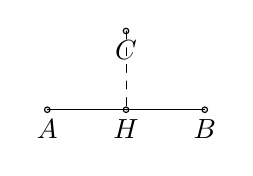
\begin{tikzpicture}
    \tkzDefPoint(0,0){A}
    \tkzDefPoint(2,0){B}
    \tkzDefPoint(1,1){C}
    \tkzDefPointBy[projection=onto A--B](C)
    \tkzGetPoint{H}
    \tkzDrawPoints(A,B,C,H)
    \tkzLabelPoints(A,B,C,H)
    \tkzDrawSegment(A,B)
    \tkzDrawSegment[dashed](C,H)
\end{tikzpicture}
        \end{center}
    }    
    \argbox{rotation 旋转}{
        \textcolor{blue}{
            \texttt{[rotation=center (旋转中心点) angle (角度)]}
        }

        \textcolor{red}{(参照点)}绕\textcolor{blue}{(旋转中心点)}旋转\textcolor{blue}{(角度)}得到的点。

        \begin{center}
        \begin{tikzpicture}
    \tkzDefPoint(0,0){O}
    \tkzDefPoint(3,0){A}
    \tkzDefPointBy[rotation=center O angle 30](A)
    \tkzGetPoint{B}
    \tkzDrawPoints(O,A)
    \tkzDrawPoints[red](B)
    \tkzLabelPoints(O,A)
    \tkzLabelPoints[above,red](B)
    \tkzDrawSegments(O,A O,B)
    \tkzMarkAngle[mark=none](A,O,B)
    \tkzLabelAngle[right](A,O,B){$30^{\circ}$}
\end{tikzpicture}
        \end{center}
    }
    \argbox{rotation in rad 弧度旋转}{
        \textcolor{blue}{
            \texttt{[rotation in rad=center (旋转中心点) angle (弧度)]}
        }

        \textcolor{red}{(参照点)}绕\textcolor{blue}{(旋转中心点)}旋转\textcolor{blue}{(弧度)}得到的点。
        
        \begin{center}
        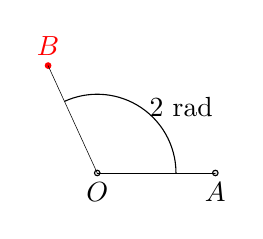
\begin{tikzpicture}
    \tkzDefPoint(0,0){O}
    \tkzDefPoint(1.5,0){A}
    \tkzDefPointBy[rotation in rad=center O angle 2](A)
    \tkzGetPoint{B}
    \tkzDrawPoints(O,A)
    \tkzDrawPoints[red](B)
    \tkzLabelPoints(O,A)
    \tkzLabelPoints[above,red](B)
    \tkzDrawSegments(O,A O,B)
    \tkzMarkAngle[mark=none](A,O,B)
    \tkzLabelAngle[right](A,O,B){2 rad}
\end{tikzpicture}
        \end{center}
    }
    \argbox{inversion 反演}{
        \textcolor{blue}{
            \texttt{[rotation in rad=center (反演中心点) through (反演圆上点)]}
        }

        \textcolor{red}{(参照点)}关于\textcolor{blue}{反演圆}的反演点,满足共线且$\textrm{OB}\times\textrm{OB'}=r^2$。
        
        \begin{center}
        \begin{tikzpicture}
    \tkzDefPoint(0,0){O}
    \tkzDefPoint(1.5,0){A}
    \tkzDefPoint(0.8,0.3){B}
    \tkzDefPointBy[inversion=center O through A](B)
    \tkzGetPoint{B'}
    \tkzDrawCircle(O,A)
    \tkzDrawPoints(O,B)
    \tkzDrawPoints[red](B')
    \tkzLabelPoints(O,B)
    \tkzLabelPoints[red](B')
    \tkzDrawSegment(B,B')
\end{tikzpicture}
        \end{center}
    }
    \auxcombox{$\backslash$tkzGetPoint 得到点}{
        ~~~在这条命令后紧跟 \texttt{$\backslash$ tkzGetPoint(结果点)} 以得到结果。
    }

\end{tcbraster}



\end{CJK}
\end{document}